\documentclass{llncs}

\usepackage[utf8]{inputenc}
\usepackage[T1]{fontenc}

\usepackage[final]{graphicx}
\usepackage{epstopdf}
\usepackage[labelsep=period]{caption}
\usepackage[hyphens]{url}

\graphicspath{{images/}}

% Закомментируйте следующую строку, если статья пишется на английском языке.
\usepackage[english,russian]{babel}

% Закомментируйте эти строки, если статья пишется на английском языке.
\def\definitionname{Определение}
\def\theoremname{Теорема}
\def\lemmaname{Лемма}
\def\notename{Примечание}

% Закомментируйте следующую строку, если статья пишется на английском языке.
\usepackage{indentfirst}

\begin{document}
	
	\title{Исследование эффективности сильно ветвящихся деревьев в задаче индексирования структурированных данных}
	
	\author{
		А.М. Ригин
	}
	
	\institute{
		ОП <<Программная инженерия>> ФКН, группа БПИ153 \\
		\email{amrigin@edu.hse.ru}
	}
	
	\maketitle
	
	
	
	\textbf{Ключевые слова:} сильно ветвящиеся деревья, $B$-деревья, $B^+$-деревья, $B^*$-деревья, индексирование структурированных данных, эффективность, сложность
	
	\section{Основные понятия и определения}
	
	\begin{itemize}
		\item \textbf{Сильно ветвящееся дерево} --- структура данных – дерево, содержащее в одном узле (вершине) более одного элемента (ключа) и более одного указателя на дочерний узел.
		\item \textbf{$B$-дерево} --- сильно ветвящееся дерево, построенное так, что если какой-то узел содержит $k$ ключей, то у данного узла $k+1$ потомков, и для любого $i$, такого, что $1\leq i\leq k+1$, верно, что все ключи в $i$-м потомке данного узла не меньше, чем $i$-й ключ данного узла, и не больше, чем $i+1$-й ключ данного узла~\cite{Kormen}.
		\item \textbf{Порядок $B$-дерева} --- такое число $t$, что для любого некорневого узла дерева верно неравенство: $t-1\leq k\leq 2t-1$, где $k$ – число ключей в узле. Корневой узел для непустого $B$-дерева содержит $1\leq k\leq 2t-1$ ключей, для пустого $B$-дерева – 0 ключей~\cite{Kormen}. B-дерево является сбалансированным деревом, поэтому его высота будет равна $O(\log_t n)$, где $n$ – число ключей в дереве~\cite{Kormen}.
		\item \textbf{$B^+$-дерево} --- модификация $B$-дерева. В $B^+$-дереве настоящие ключи хранятся лишь в листьях дерева, а во внутренних узлах хранятся лишь ключи-маршрутизаторы, необходимые для поиска по дереву. Листья в B+-дереве содержат $t\leq n\leq 2t$ ключей, где $t$ – порядок дерева, ограничения для внутренних узлов такие же, как и в $B$-дереве. Деление листьев происходит поровну на две части, крайний ключ из левой половины делимого узла копируется в родительскую вершину в качестве ключа-маршрутизатора аналогично перемещению медианы для обычного деления, деление внутренних узлов происходит так же, как и в $B$-дереве~\cite{Kerttu}.
		\item \textbf{$B^*$-дерево} --- модификация $B$-дерева. Каждый узел заполняется не менее, чем на 2 / 3, а не 1 / 2, как в $B$-дереве. По этой причине, вместо традиционного разбиения узла, происходит перераспределение ключей между соседними узлами-потомками, либо, если нет незаполненных соседей, то узел разбивается на три (а не на две, как в $B$-дереве, части) части~\cite{Nist}.
	\end{itemize}
	
	\section{Значимость работы}
	
	Значимость данной работы связана с тем, что сильно ветвящиеся деревья активно используются в различных задачах, связанных с индексированием структурированных данных для снижения времени, затрачиваемого на выполнение различных поисковых операций, например, в системах управления базами данных (СУБД).
	
	\section{Цель работы}
	
	Целью работы является исследование эффективности сильно ветвящихся деревьев, структура которых задаётся определённым набором параметров, в задаче индексирования структурированных данных, в том числе, измерение сложности основных операций (с экспериментальной оценкой занимаемой памяти) с такими деревьями при их различных параметрах построения дерева.
	
	\section{Задачи работы}
	
	Задачами данной работы являются:
	
	\begin{enumerate}
		\item обзор литературы и других работ в данной области;
		\item построение теоретической модели;
		\item реализация структур данных --- $B$-дерева, $B^+$-дерева и $B^*$-дерева на языке C++, а также инструмента для проведения экспериментов и вывода их результатов;
		\item построение схемы экспериментов, в том числе, создание набора различных изменяемых параметров построения $B$-дерева, $B^+$-дерева и $B^*$-дерева для проведения различных экспериментов;
		\item проведение экспериментов (измерений сложности основных операций с такими деревьями --- поиска, вставки и удаления элементов – при различных параметрах построения дерева, с экспериментальной оценкой занимаемой памяти) согласно построенной схеме экспериментов;
		\item интерпретация полученных результатов, получение выводов.
	\end{enumerate}
	
	\section{Ожидаемые результаты}
	
	Ожидаемыми результатами данной работы являются:
	
	\begin{enumerate}
		\item проведённый обзор литературы и других работ в данной области;
		\item построенная теоретическая модель;
		\item реализованные на языке C++ структуры данных – $B$-дерево, $B^+$-дерево и $B^*$-дерево и разработанный инструмент для проведения экспериментов и вывода их результатов;
		\item построенная схема экспериментов, в том числе, созданный для проведения различных экспериментов набор различных изменяемых параметров построения $B$-дерева, $B^+$-дерева и $B^*$-дерева;
		\item результаты проведённых экспериментов – измеренное время выполнения основных операций с такими деревьями – поиска, вставки и удаления элементов – при различных параметрах построения дерева (с экспериментальной оценкой занимаемой памяти);
		\item интерпретация полученных результатов экспериментов и выводы на их основе.
	\end{enumerate}
	
	\section{Предварительные результаты}
	
	\subsection{Теоретические оценки сложности основных операций с деревом}
	
	\subsubsection{$B$-дерево:}
	
	$t$ --- степень дерева, $n$ --- число ключей в дереве.
	
	\begin{enumerate}
		\item поиск --- $O(t\log_t n)$ по времени~\cite{Kormen}, $O(t\log_t n)$ по памяти (для реализации поиска при помощи рекурсии), $O(t)$ по памяти (для реализации поиска при помощи цикла), $O(\log_t n)$ дисковых операций;
		\item разбиение --- $O(t)$ по времени, $O(t)$ по памяти, $O(1)$ дисковых операций;
		\item вставка --- $O(t\log_t n)$ по времени, $O(t\log_t n)$ по памяти (для реализации вставки при помощи рекурсии), $O(t)$ по памяти (для реализации вставки при помощи цикла), $O(\log_t n)$ дисковых операций;
		\item удаление --- $O(t\log_t n)$ по времени~\cite{Kormen}, $O(t\log_t n)$ по памяти, $O(\log_t n)$ дисковых операций~\cite{Kormen}.
	\end{enumerate}
    
    \subsubsection{$B^+$-дерево:}
    
    Асимптотика у всех основных операций совпадает с асимптотикой соответствующих операций в B-дереве. Средняя вычислительная сложность поиска должна увеличиться, но теперь известно, что ключ гарантированно в листе дерева (если находится в дереве). Средняя вычислительная сложность удаления должна уменьшиться.
    
    \subsubsection{$B^*$-дерево:}
    
    Асимптотика у всех основных операций совпадает с асимптотикой соответствующих операций в B-дереве. Фактическая сложность на деле должна отличаться от таковой в B-дереве, поскольку из-за того, что каждый узел более заполнен, высота дерева будет меньше, но будет увеличена линейная составляющая.
	
	\subsection{Примеры эмпирических оценок сложности основных операций с деревом}
	
	В качестве примера эмпирической оценки сложности поиска в дереве на рис. ~\ref{fig:BTreeSearchTime} и рис. ~\ref{fig:BPlusTreeSearchTime} приведены графики времени (сек) поиска всех 1136 вхождений некоторого значения ключа в соответственно $B$-дереве и $B^+$-дереве, построенном на выборке данных, состоящей из 150291 объектов, для порядков дерева от 50 до 2050 включительно.
	
	На данных графиках видно, что $B^+$-дерево даёт лучший результат для поиска, чем $B$-дерево, хотя, согласно теоретическая оценке, должно быть наоборот. Это может быть связано с тем, что поиск ведётся для 1136 вхождений ключа за один проход по дереву, и, благодаря тому, что в $B^+$-дереве все настоящие ключи находятся только в листьях дерева, в нём приходится обходить меньшее число вершин.
	
	\begin{figure}[h!]
		\centering
		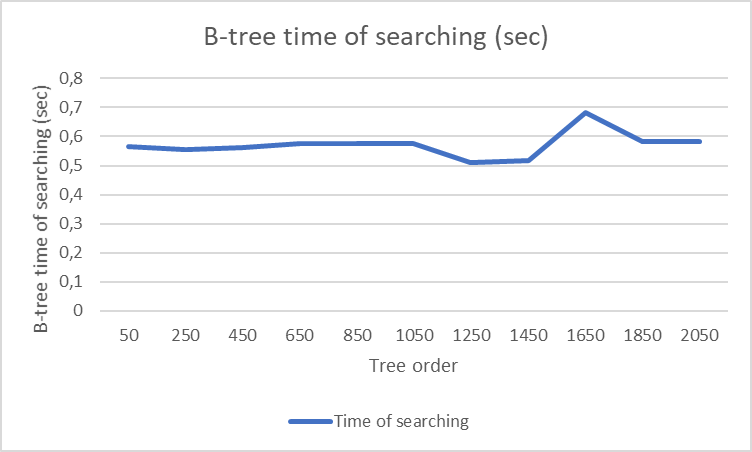
\includegraphics[width=7.5cm]{BTreeSearchTime}
		\caption{Время (сек) поиска всех 1136 вхождений ключа в $B$-дереве со 150291 элементом при порядке дерева от 50 до 2050}
		\label{fig:BTreeSearchTime}
	\end{figure}
    
    \begin{figure}[h!]
    	\centering
    	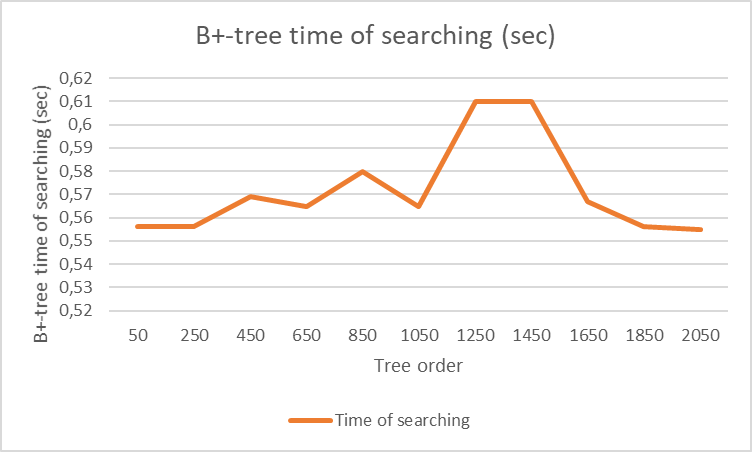
\includegraphics[width=7.5cm]{BPlusTreeSearchTime}
    	\caption{Время (сек) поиска всех 1136 вхождений ключа в $B^+$-дереве со 150291 элементом при порядке дерева от 50 до 2050}
    	\label{fig:BPlusTreeSearchTime}
    \end{figure}
	
	\section{Список используемых источников}
	
	\begingroup
	\renewcommand{\section}[2]{}
	\begin{thebibliography}{}
		\bibitem{Kormen}
		Т. Кормен, Ч. Лейзерсон, Р. Ривест, К. Штайн. Алгоритмы: построение и анализ. 3-е изд. --- М.: ИД "Вильямс". --- 2013. --- 1324 с.
		\bibitem{Knut}
		Кнут Д.Э. Искусство программирования. Том 3. Сортировка и поиск. 2-е изд. --- М.: ИД "Вильямс". --- 2002. --- 800 с.
		\bibitem{Bayer}
		Bayer R., McCreight E. Organization and Maintenance of Large Ordered Indexes // Acta Informatica. --- 1972, V. 1. --- P. 173-189
		\bibitem{Washam}
		Washam J. An Astounding Example of Efficiency with B-Trees [Electronic Source] // Startup Nextdoor. --- URL: https://startupnextdoor.com/an-astounding-example-of-efficiency-with-b-trees/ [Date: 2017/12/07]
		\bibitem{Kerttu}
		Kerttu Pollari-Malmi. $B^+$-trees [Electronic Source] --- URL: https://www.cs.helsinki.fi/u/mluukkai/tirak2010/B-tree.pdf [Date: 2017/12/07]
		\bibitem{Nist}
		$B^*$-tree [Electronic Source] // NIST Dictionary of Algorithms and Data Structures --- URL: https://xlinux.nist.gov/dads/HTML/bstartree.html [Date: 2017/12/23]
	\end{thebibliography}
	
\end{document}